
Cilk was originally developed in the 1990’s at Massachusetts Institute of Technology. It was
later productized and commercialized by a spinoff company, Cilk Arts. During the 2000’s Cilk
Arts targeted the high performance and highly parallel multi-core computer market, which were emerging as consumer commodity products at the time. Intel acquired Cilk Arts in 2009 and codeveloped Cilk’s enhancements with its hardware. The current version of Cilk being investigated in this report is Cilk Plus. This is Intel’s development branch of Cilk that is tuned to Intel’s C/C++ Compiler; however, it is also available in GCC versions 4.9 and above. In this
paper, the terms Cilk and Cilk Plus will be used interchangeably, despite their semantic
differences.

Cilk is a faithful extension of C/C++. One of the key principles of Cilk is that the
programmer should be responsible for exposing the parallelism of the algorithm and should
identify those elements that lend themselves to be parallelized. The scheduling and execution
model should be left to the processor hardware. This philosophy is important in the sense that the degree of parallelism is ultimately determined by the hardware and system resources. Such an approach to parallelism is ideal when trying to measure and calculate the theoretical growth of certain algorithms that lend themselves to be parallelized. The Cilk framework can leverage the hardware capabilities of the system by having the programmer expose as much parallelism in the algorithms using Cilk keywords.


\subsection{How Cilk Works}
The Cilk scheduler, which is what Cilk uses to divide work during execution among multiple processors, is based on the concept of “work-stealing”. Specifically, Cilk uses greedy work-stealing algorithms to assign specific function tasks to available cores. The programmer exposes those functions that are parallelizable using a variety of keywords. The main two are the “spawn” and “sync” keywords; however, Cilk has expanded its constructs to include the \texttt{cilk\_for} construct.

Cilk follows certain rules regarding spawned functions’ parent-child relationships. For example, a child cannot view a sibling’s data, only the parent’s. However, when the child finishes executing or is idle a processor will try to “steal” work from a sibling. This is achieved with “cactus stacks”. In these kinds of stacks, the activation frames of Cilk procedures are pushed onto the stack and idle processors try to take the most recently pushed work available.

The programmer will signal to the compiler that a function is a Cilk function with the keyword cilk in the function declaration. In the body of the function the keyword “spawn” is used to signal that a parallelizable procedure is to be used and that a parent-child relationship exists. The parent will not be able to return until all spawned children have “sync[ed]”. If this parallelism is done in a recursive fashion, deep parent-child functions will exist giving it the “cactus” appearance.


\subsection{Cilk Implementation: Recursive}

The classic Cooley-Tukey FFT algorithm makes use of recursion to reduce computation time of FFT decomposition by splitting up the even and odd terms. Cilk parallelism can be exposed in recursive algorithms with ease by utilizing the \texttt{cilk\_spawn} and \texttt{cilk\_sync} keywords. Since the even and odd terms of the FFT are independent a CPU with sufficient resources will be able to compute these in parallel given cilk’s spawn routines. When both spawned children are done they must be synced to ensure coherent programming order.

From a programming point of view, cilk is a very easy tool for the programmer to use since the recursive routine can first be written without any cilk constructs. When functional correctness is established, the cilk keywords may be introduced. Cilk includes tools to make sure that after the introduction of all cilk constructs no race conditions exist, which could break functional correctness.

In the Cooley-Tukey FFT algorithm, the merging step that occurs after the divide and conquer steps are complete can also expose parallelism to cilk. In our implementation this step is called via the \texttt{cilk\_combine()} function. Cilk spawns two threads of \texttt{cilk\_combine()} with arrays of half the size. When the sub-arrays reach below a certain threshold of \texttt{cilk\_max\_recombine}, the \texttt{cilky\_combine()} function is called. This function uses the \texttt{cilk\_for} construct to parallelize work. Another approach that is different from the \texttt{cilk\_for} for the array additions of the two sections of the FFT (Even and Odd) that was not implemented would have been to use the Cilk Array notation, which would allow the compiler/processor to vectorize the additions and expose parallelism differently than with the \texttt{cilk\_for}. 

From a parallel algorithms perspective it is interesting to note the performance impact of the value of \texttt{cilk\_max\_recombine}. Figure \ref{cilk_max_recombine} shows that as the number of elements of the FFT grows, there is a noticeable performance gap between the two cilk recursive runs where the only change is in the value of \texttt{cilk\_max\_recombine} (value of 1 vs. 128). A value of 128 represents fewer threads processing more values in \texttt{cilky\_combine()} as compared to a value of 1 where more threads are processing fewer elements in parallel. This is akin to the cascaded parallel algorithm technique of splitting up the groups of elements a certain way to achieve a work-optimal solution. 

\begin{figure}
\center
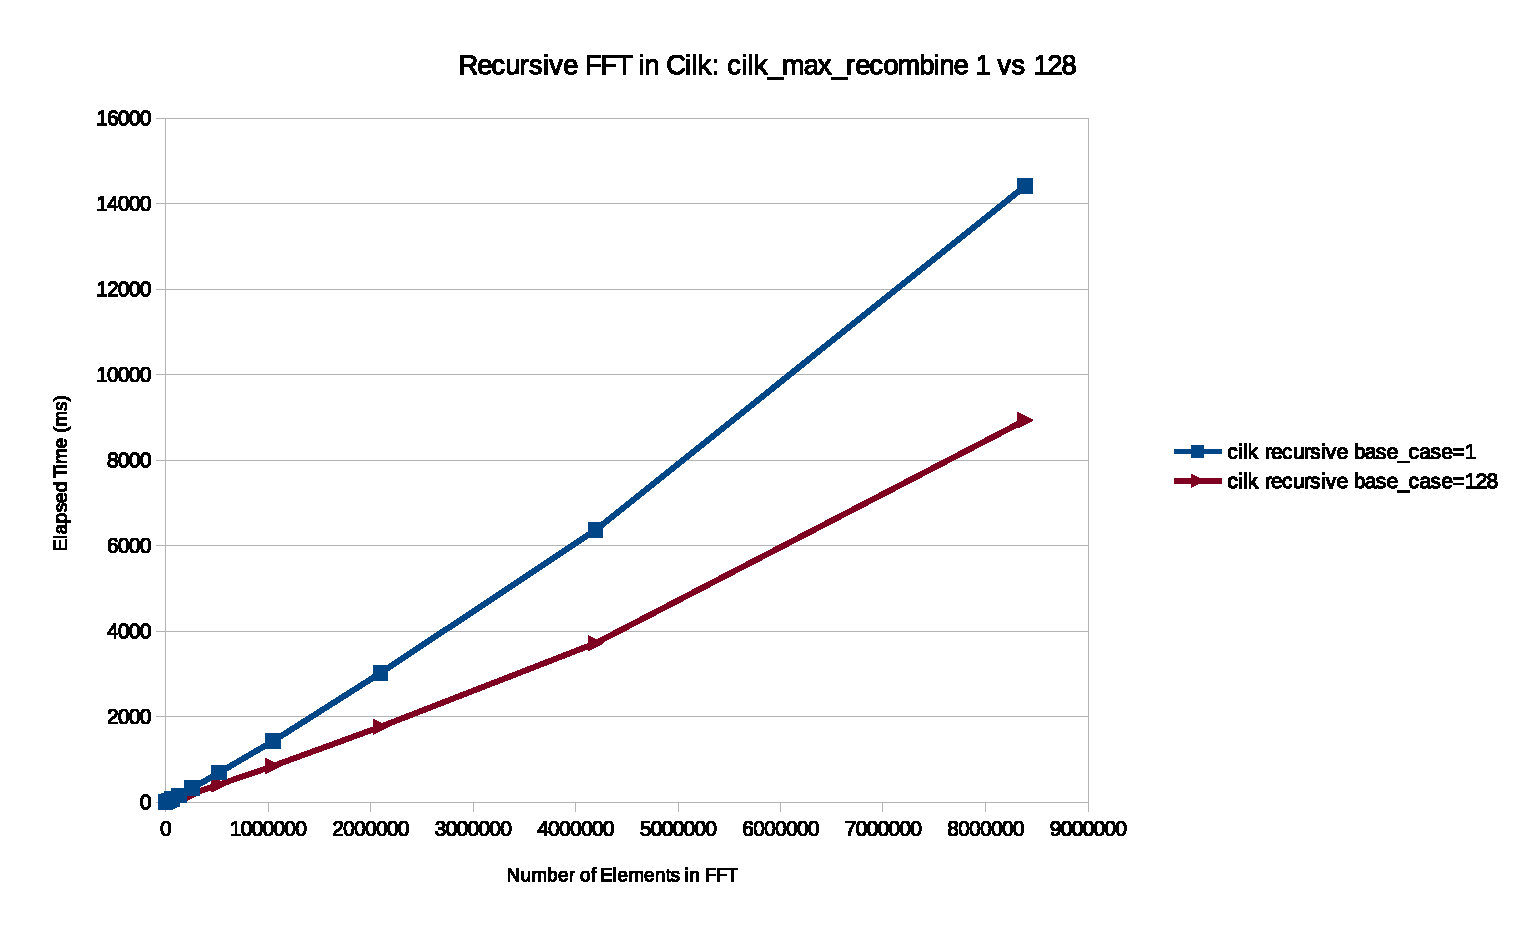
\includegraphics[scale=0.55]{img/cilk_max_recombine.eps}
\caption{Graph comparing the two cilk recursive runs with values of \texttt{cilk\_max\_recombine}=1,128} 
\label{cilk_max_recombine}
\end{figure}

It should be noted that the recursive solution is still of time-complexity $O(n * log(n))$ as the algorithm is not changed. However, the cilk constructs expose potential parallelism which means that overall running time is decreased given system resources. 



\subsection{Cilk Implementation: Iterative}
In a similar fashion as the recursive cilk implementation, the first step of a cilk iterative solution is to attain functional correctness of an iterative implementation sans cilk. The cilk constructs are added later. The iterative solution relies of loops to calculate the FFT. Modern processors equipped with Out of Order Execution engines are able to optimize and run these types of programs faster than the recursive solution that is more stack-intensive and contains more control transfer instructions. It is not a surprise that even the non-parallel iterative implementation is faster than the recursive one especially as the number of elements to process increases. This performance difference is shown in Figure \ref{iterative_recursive_non_cilk}.

\begin{figure}
\center
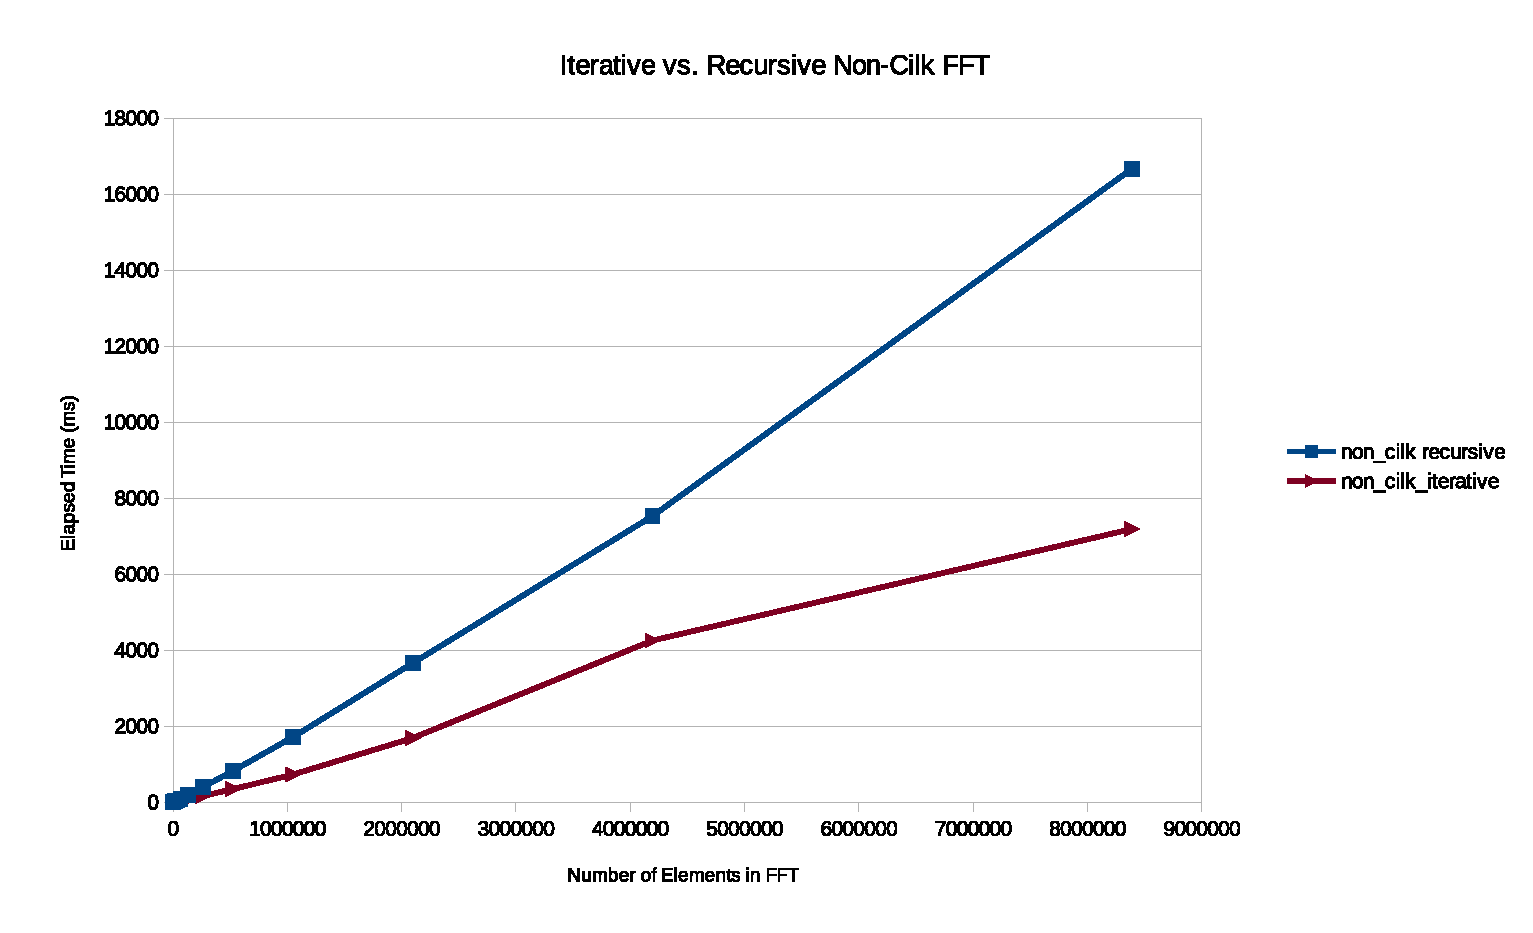
\includegraphics[scale=0.6]{img/iterative_recursive_non_cilk.eps}
\caption{Graph comparing the performance of the iterative and recursive non-cilk (C++) FFT algorithms} 
\label{iterative_recursive_non_cilk}
\end{figure}

The introduction of the \texttt{cilk\_for} construct allows for loops with independent operations to run in parallel. Replacing one for with a \texttt{cilk\_for} in the \texttt{cilk\_transform\_iter()} function results in a dramatic performance boost as can be seen in the graph of figure \ref{iterative_fft}. 
Similarly to the recursive cilk implementation, the cilk iterative algorithm is still of the same complexity, $T(n) = O(n * log(n))$, but is faster due to the exposed parallelism. 

\begin{figure}
\center
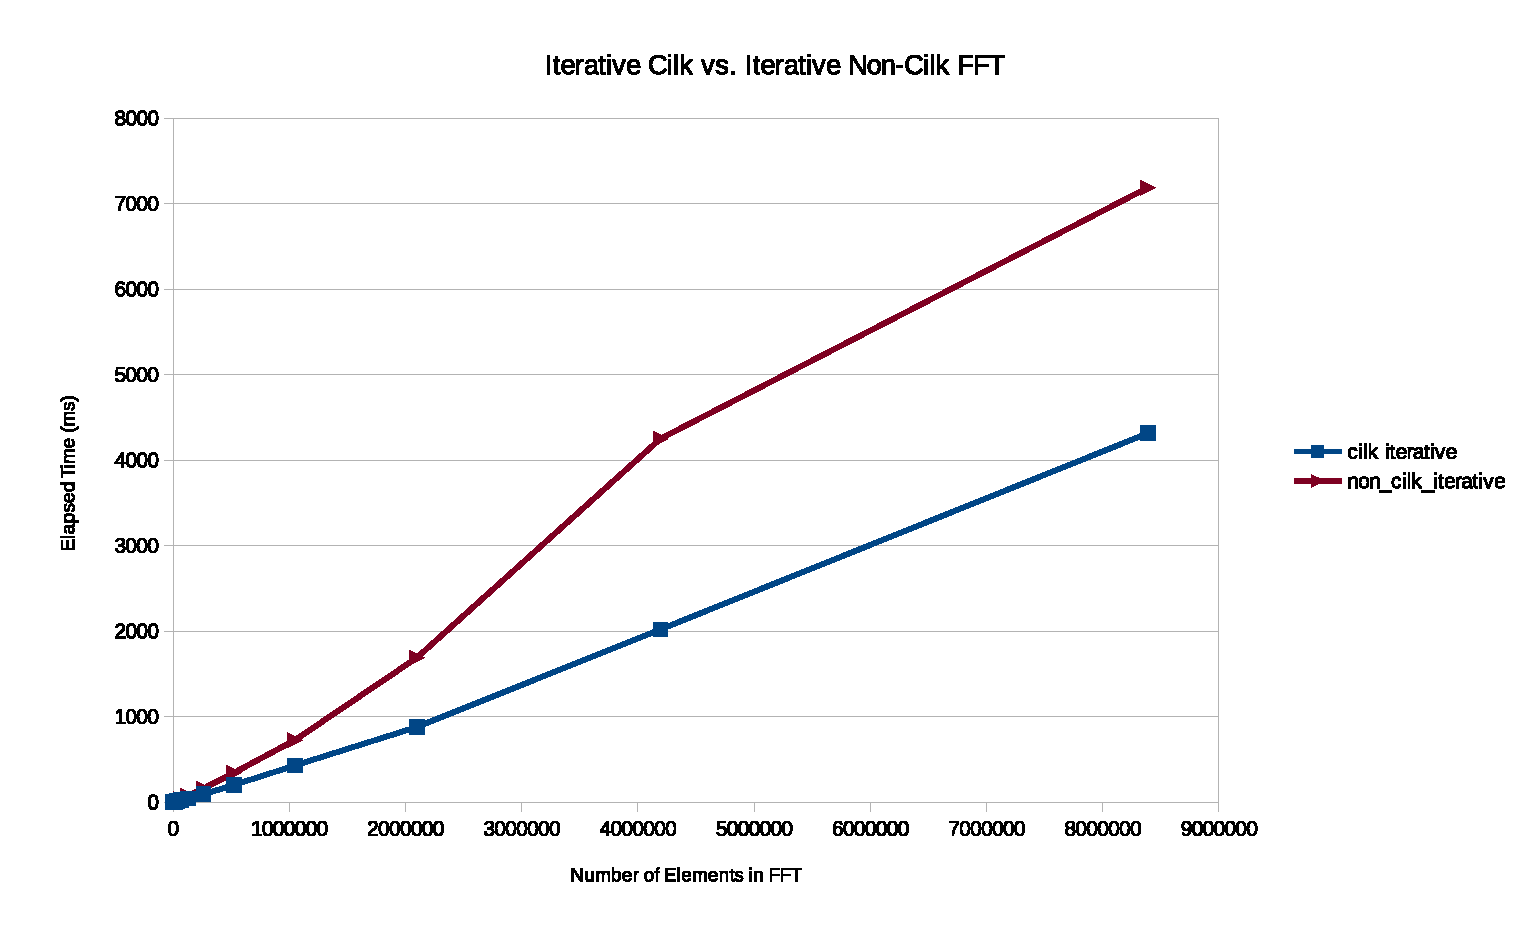
\includegraphics[scale=0.6]{img/iterative_fft.eps}
\caption{Graph comparing the performance of the iterative cilk and non-cilk (C++) FFT algorithms} 
\label{iterative_fft}
\end{figure}

\subsection{Cilk Analysis}
As can be seen in the graph of figure \ref{fft_cilk_cpp}, the performance differences between the five different algorithms becomes clear when processing at least 2\textsuperscript{10} elements. The non-cilk C++ recursive algorithm is the slowest performance-wise. The recursive recursive  implementation that uses a value of \texttt{cilk\_max\_recombine} value of 1 is faster than the non-cilk version, but not by much. An interesting observation is that the cilk recursive algorithm with a \texttt{cilk\_max\_recombine} value of 128 is faster than the version that uses a value of 1 for all values save some outliers. In fact, it is close to \( \frac{2}{3} \) the completion time of the \texttt{cilk\_max\_combine} value of 1.

\begin{figure}
\center
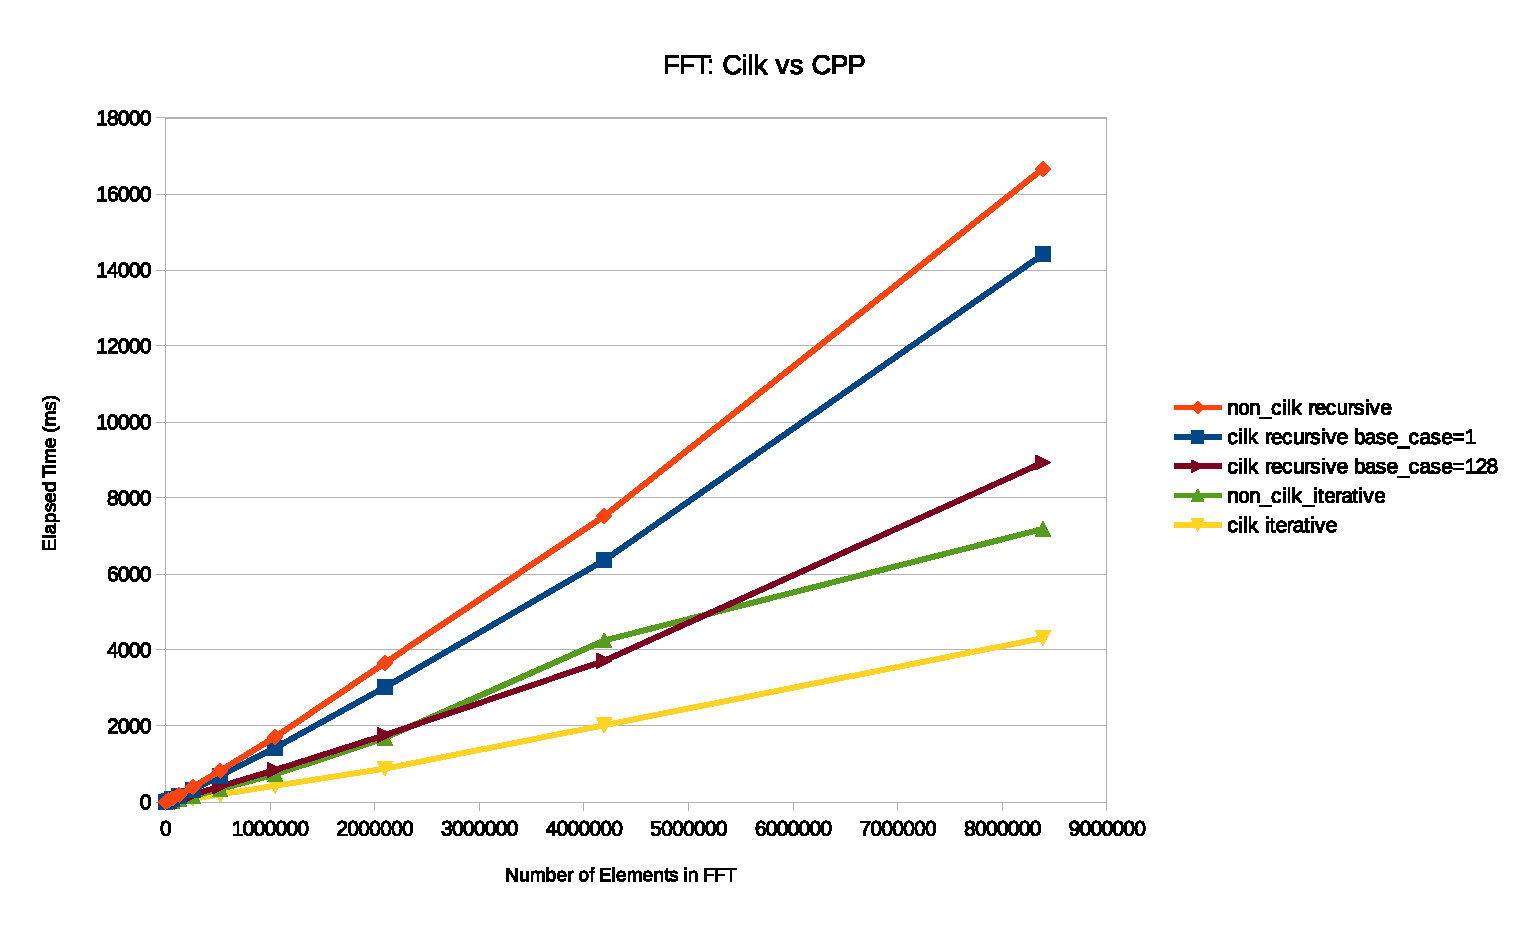
\includegraphics[scale=0.6]{img/fft_cilk_cpp.eps}
\caption{Graph comparing the performance of all FFT algorithms, cilk and C++} 
\label{fft_cilk_cpp}
\end{figure}

Moreover, the iterative cilk implementation is by far the highest performing algorithm. It is about 1.6x times faster than the non-cilk version for large values. Another observation worth noting is that the iterative non-cilk solution is ~2.3x faster than its non-cilk version. This relationship is similar between the cilk iterative implementation and the recursive cilk \texttt{cilk\_max\_recombine}=128 solution (~2x performance gains), while it grows to as much as ~3.3x as compared to the recursive cilk \texttt{cilk\_max\_recombine}=1 solution . 

Cilk does provide built-in ways to adjust the “grain-size” of the threads. This was not used in this project; however, from the curves of the graph in figure \ref{cilk_max_recombine} it is obvious that a lot of performance improvement can be gained with calibration of the number of threads cilk uses. 

The parallelism gained by cilk comes at the cost of memory (space complexity) usage. Inherently, it is very difficult to measure stack usage by cilk since it manipulates the stack so much to achieve parallelism that any attempts to trace stack usage affects cilk performance negatively. However, heap usage is easy to measure using the program profiling tool Valgrind with the heap profiler massiff. As can be seen from images in figure \ref{fig:masiff}, the iterative cilk solution that uses the \texttt{cilk\_for} construct does not use much more heap space than the non-cilk iterative one. This may be due to cilk’s internal vectorization instead of the spawn/sync mechanism. The recursive cilk solution uses more heap space than the non-cilk version (~41MB vs. ~28MB). 

\begin{landscape}
\thispagestyle{empty}
\begin{figure}
\centering
        \begin{subfigure}[b]{0.65\textwidth}
            \center
            \includegraphics[width=\textwidth]{img/fft_iter_cilk.png}
            \caption{Heap memory usage of iterative cilk algorithm}
            \label{fig:heap_iter_cilk}
        \end{subfigure}%
        \begin{subfigure}[b]{0.65\textwidth}
            \center
            \includegraphics[width=\textwidth]{img/fft_iter_cpp.png}
            \caption{Heap memory usage of iterative C++ algorithm}
            \label{fig:heap_iter_cpp}
        \end{subfigure}%
        \vskip\baselineskip
        \begin{subfigure}[b]{0.65\textwidth}
            \center
            \includegraphics[width=\textwidth]{img/fft_rec_cilk.png}
            \caption{Heap memory usage of recursive cilk algorithm}
            \label{fig:heap_rec_cilk}
        \end{subfigure}%
        \begin{subfigure}[b]{0.65\textwidth}
            \center
            \includegraphics[width=\textwidth]{img/fft_rec_cpp.png}
            \caption{Heap memory usage of recursive C++ algorithm}
            \label{fig:heap_rec_cpp}
        \end{subfigure}
        \caption{Valgrind's masiff Heap tracer for cilk vs C++}\label{fig:masiff}
\end{figure}
\end{landscape}